
\par \textit{Machine learning} is a subfield of \textit{Artificial Intelligence}, which involves algorithms that enable automatic learning of tasks based on data. Unlike classical programming, which involves giving instructions and input data to a computer and producing output data, machine learning aims to produce the instructions or rules used for a task as the result, when the input and corresponding output data is provided to a computer.

\par \textit{Deep Learning}, a subfield of Machine Learning has been growing popular in recent years, owing to their performance over traditional machine learning techniques without the need for intensive feature engineering by practitioners; deep learning models involve building up successive layers of increasingly meaningful representations automatically, allowing them to be rich and expressive with information. Different forms of deep learning models, including dense or fully connected layers, convolutional networks, recurrent networks and others have been applied to a variety of tasks which traditional algorithms have failed to address. Among different deep learning models in the literature, \textit{transformers} are gaining traction in a variety of tasks, including sequence to sequence tasks like machine translation, natural language generation and understanding, and recently, computer vision.

\par Transformers were introduced by Vaswani \textit{et al} in \cite{tfm}. The transformer architecture is shown in \ref{fig:transformer}. It consists of encoder layers which use \textit{multi-head self-attention} on input tokens followed by fully connected layers. The decoder layers use the output tokens and representations from encoder layers in a \textit{multi-head cross-attention} block followed by fully connected layers. This architecture has been adapted by various other models to serve a variety of tasks.

\begin{figure}[h]
\centering
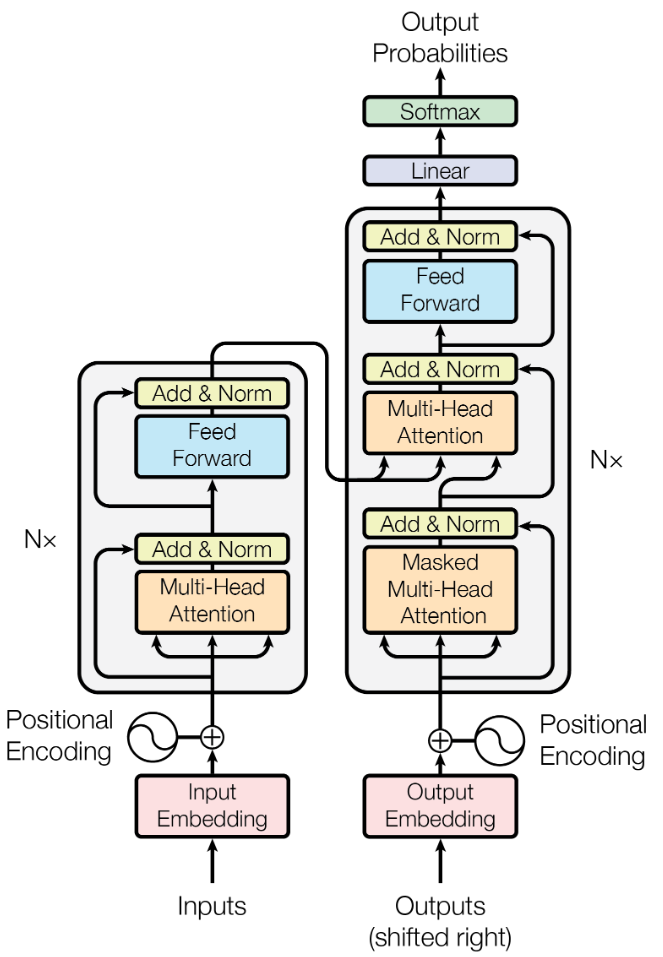
\includegraphics[width=0.5\linewidth]{assets/img/transformer.png}
\caption{The Transformer architecture. Image courtesy \cite{tfm}}
\label{fig:transformer}
\end{figure}